%%%%%%%%%%%%%%%%%%%%%%%%%%%%%%%%%%%%%%%%%%%%%%%%%%%%%%%
\begin{frame}

\frametitle{Small Example}

A small example has been made available on GitHub:  \href{http://www.github.com/rwanwork/Snakemake-Example/}{http://www.github.com/rwanwork/Snakemake-Example/}.
\vs

Performs simple tasks:
\begin{enumerate}
  \item Download an example from the University of California of Irvine's Machine Learning Repository.
  \item Count the number of lines in the data file.
  \item Randomize the lines of the data file.
  \item Compress the permuted data file.
  \item Calculate the MD5 message digest of the permuted data file.
\end{enumerate}

\end{frame}


%%%%%%%%%%%%%%%%%%%%%%%%%%%%%%%%%%%%%%%%%%%%%%%%%%%%%%%
\begin{frame}

\frametitle{Small Example}

The dependency graph with two data sets looks like this:
\begin{figure}
  \centering
  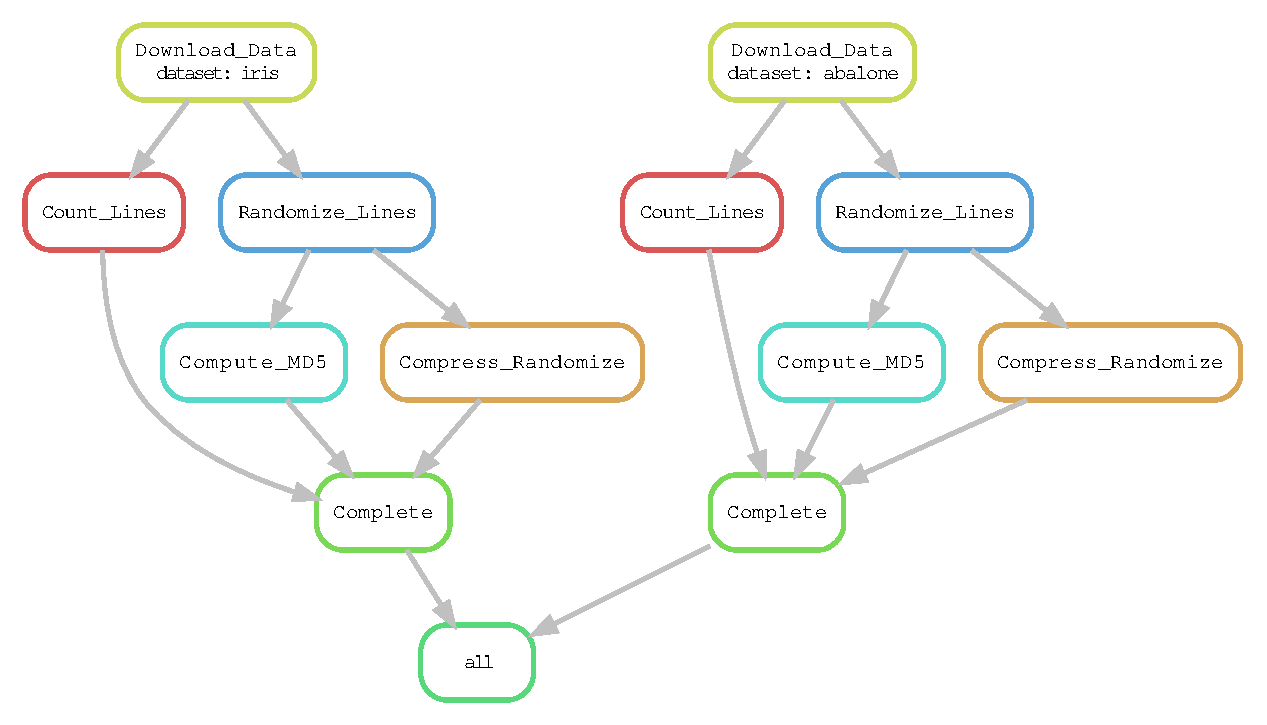
\includegraphics[width=\linewidth]{example/graph}
\end{figure}

\end{frame}


%%%%%%%%%%%%%%%%%%%%%%%%%%%%%%%%%%%%%%%%%%%%%%%%%%%%%%%
\begin{frame}

\frametitle{Other Works}

\begin{figure}
  \centering
  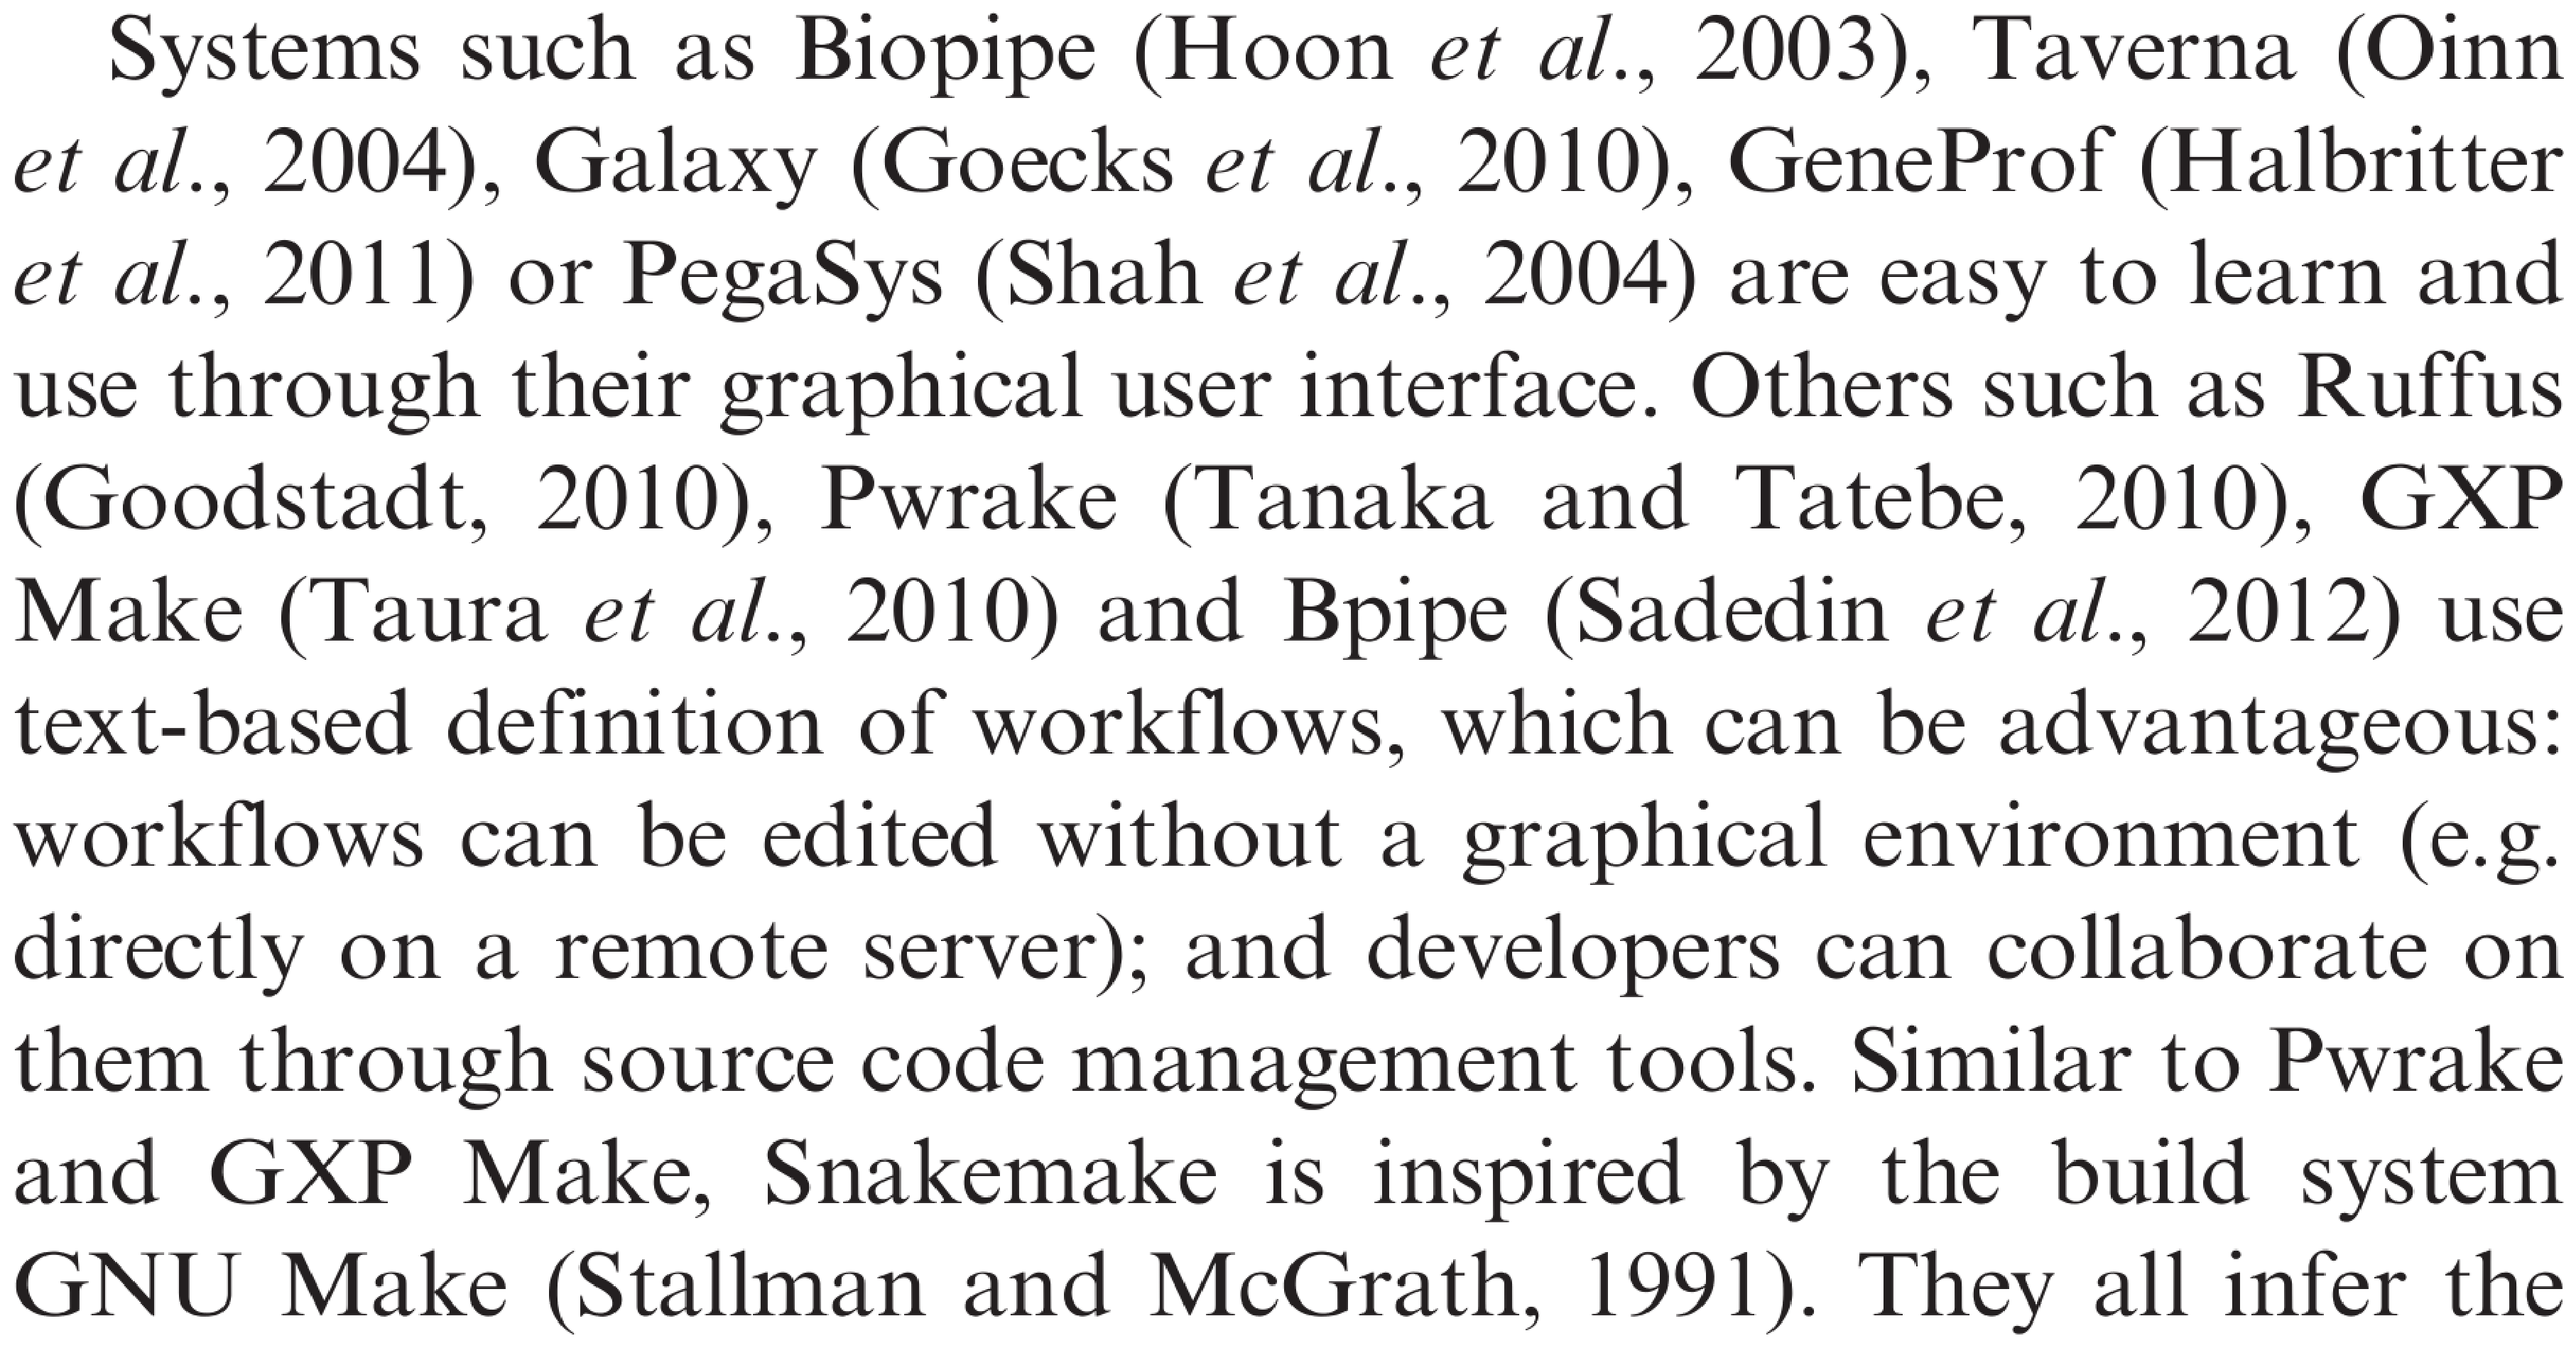
\includegraphics[width=\linewidth]{conclude/related}
\end{figure}

{\figsource{From the Snakemake paper}}

\end{frame}


%%%%%%%%%%%%%%%%%%%%%%%%%%%%%%%%%%%%%%%%%%%%%%%%%%%%%%%
\begin{frame}

\frametitle{Further Information}

More information is available from the developer:
\begin{description}
  \item[Documentation] \href{https://snakemake.readthedocs.io/en/stable/}{https://snakemake.readthedocs.io/en/stable/}
  \item[Manuscript] In Bioinformatics journal\footnote{\href{https://academic.oup.com/bioinformatics/article/28/19/2520/290322}{https://academic.oup.com/bioinformatics/article/28/19/2520/290322}}
  \item[Source] \href{https://bitbucket.org/snakemake/snakemake.git}{https://bitbucket.org/snakemake/snakemake.git}
\end{description}

\end{frame}


